\chapter{Qu'est-ce qu'un plasma ? De l'exemple du vent solaire à la problématique d'étude}
\renewcommand\partie{\Partie\ Chapitre \thechapter}
\label{ch-02}

%\medskip
\minitoc  

\bigskip

Dans le Chapitre \ref{ch-01}, nous avons défini de manière hydrodynamique (HD) ce qu'est la turbulence grâce à la théorie des lois exactes de Kolmogorov. Ce sera le seul chapitre placé dans le domaine hydrodynamique. Dans l'univers visible (ou baryonique), la matière est majoritairement sous forme de plasma que l'on ne peut décrire par les équations de Navier-Stockes incompressibles seules. On s'intéressera donc à la turbulence dans un plasma. 

Ici, nous allons définir ce qu'est un plasma et comment le décrire, puis nous aborderons les questions ouvertes, motivations des travaux décrits dans ce mémoire. 

\section{Les plasmas, état de la matière} \label{sec-021}

La matière peut être décrite comme des poupées russes constituées de particules de tailles diverses, allant des atomes et molécules aux quarks en passant par les protons et les électrons qui sont des particules chargées positivement et négativement. Elle peut aussi être décrite en fonction de son état : solide, liquide, gaz et plasma. 

Les états solide, liquide et gaz sont les états les plus reconnus dans notre quotidien. Ils sont généralement constitués de molécules ou d'atomes neutres ne portant pas de charge électrique. Pourtant, ces états sont des exceptions dans l'univers, où la matière est majoritairement à l'état de plasma : les atomes y sont dissociés en particules chargées, ions, protons et électrons. Ces particules induisent un champ électromagnétique s'il n'y en a pas originellement. Le plasma sera entretenu par les interactions entre les champs électrique et magnétique et les particules. \textbf{\emph{Un plasma est donc un milieu constitué de particules chargées et de champs électrique et magnétique en étroite interaction.}}

On peut aussi en reconnaître dans notre quotidien, le plus souvent ils brillent ! Par exemple, les éclairs, les aurores, les flammes, les néons, les étoiles et les nébuleuses. Ils forment finalement la grande majorité de la matière présente dans l'univers, du centre des planètes au milieu intergalactique. Pour les étudier, on a deux possibilités : les créer en laboratoire ou s'immerger dedans. Dans le deuxième cas, peu sont réellement accessibles, beaucoup étant trop furtif (les éclairs), trop lointains (les nébuleuses) ou trop extrêmes (le soleil) pour y envoyer des appareils de mesure. Parmi les plasmas naturels accessibles, l'espace interplanétaire est roi. Véritable laboratoire [\cite{bruno_solar_2005}], on y envoie régulièrement des sondes et satellites. La dernière sonde en date est \ac{JUICE} lancée le 14 avril 2023 en direction du système lunaire de Jupiter. 

Dans l'espace interplanétaire, on trouve différents types de plasmas. Si l'on décolle de la surface d'une planète telle que la Terre, on commencera par traverser l'atmosphère constituée de gaz neutre. Puis, on atteindra l'ionosphère, un plasma d'ions lourds et impactés par le champ magnétique planétaire. En s'écartant un peu plus, on s'immergera dans la magnétosphère constituée d'ions légers (principalement des protons) et d'électrons, toujours sous l'influence du champ planétaire. En partant du Soleil, on peut aussi définir différentes couches, la chromosphère, une couche fine gazeuse, puis la couronne solaire, un plasma s'étendant sur une quinzaine de rayons solaires et enfin l'héliosphère dans lequel baignent les planètes. Le Soleil y éjecte continuellement un plasma : le vent solaire.
Le mouvement des planètes dans le vent solaire vient former un arc de choc les précédant. Entre cet arc et la magnétosphère, le vent solaire est choqué. Cette région, dominée par le champ magnétique interplanétaire, est la magnétogaine. La \figref{fig:régions} illustre quelques-unes de ces différentes régions. D'autres régions plus spécifiques existent, mais on se contentera de ce niveau de description, le vent solaire étant notre principal objet d'étude. 
\begin{figure}[!ht]
 \centering
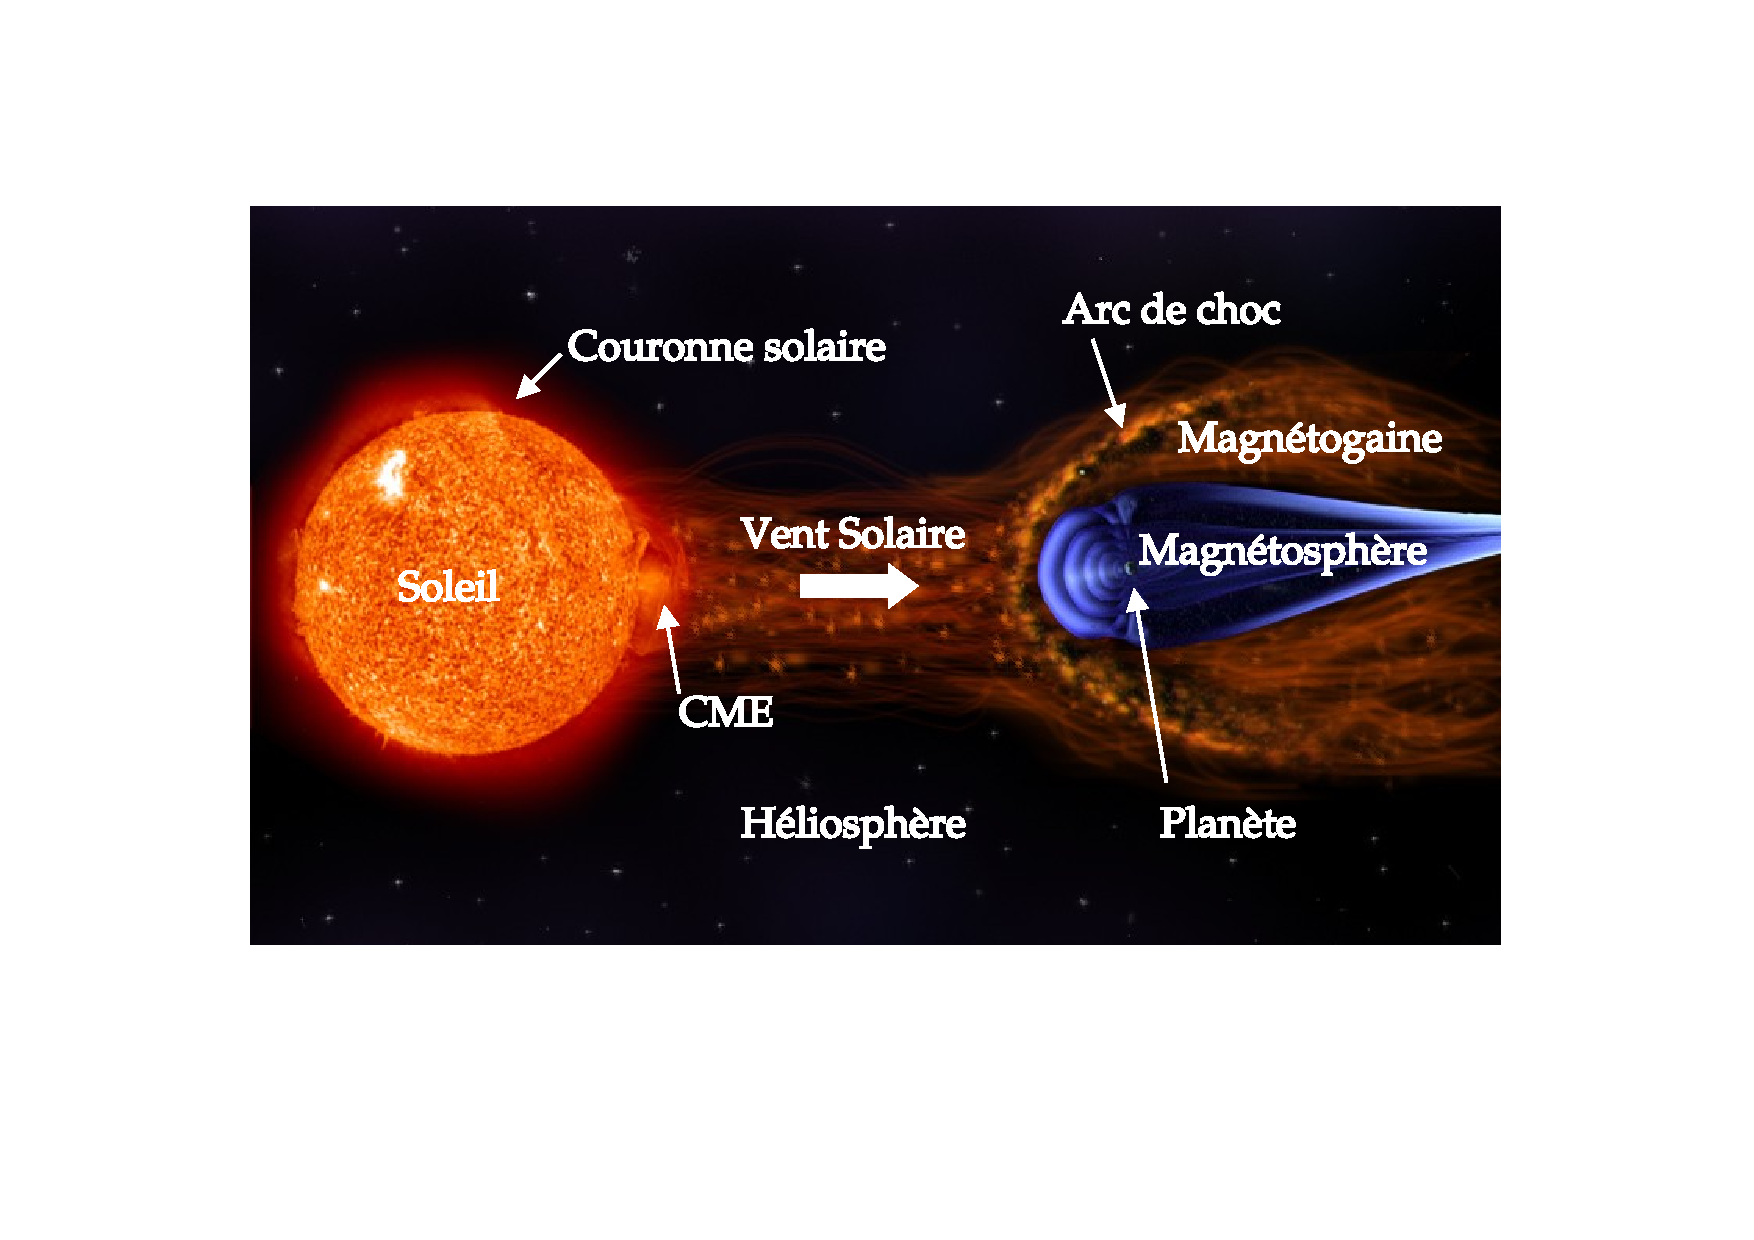
\includegraphics[width=\linewidth,trim=4cm 5cm 4cm 4cm, clip=true]{./Part_0/images/schemes_heliosphere}
\cprotect\caption{Exemples de plasmas spatiaux. \acs{CME} signifie éjections de masse coronale. Crédits de l'image initiale : Institut royal d'Aéronomie Spatiale de Belgique (page web \verb|www.aeronomie.be|).}
\label{fig:régions}
\end{figure}
Le vent solaire est par exemple traversé par \ac{PSP} en orbite autour du Soleil, cette mission lancée par l'agence spatiale américaine \acs{NASA} en 2018 s'approche petit à petit du Soleil afin de <<toucher>> la couronne. La mission \ac{MMS} en orbite autour de la Terre explore le vent solaire, la magnétogaine et la magnétosphère. Nous reparlerons plus en détail de ces deux missions dans le Chapitre \ref{ch-14}. 

\section{Le vent solaire, source de questions ouvertes et problématique d'étude} \label{sec-022}

Le vent solaire est un plasma extrêmement dilué, peu collisionnel et turbulent, constitué essentiellement d'ions légers ou protons (hydrogène, hélium chargés) et d'électrons interagissant avec le champ magnétique du Soleil. En fonction de l'activité cyclique et des latitudes du Soleil, il peut être rapide ($v_{SW} \sim \SI{800}{km/s}$) ou lent ($v_{SW} \sim \SI{400}{km/s}$) et parcouru par des structures à grandes échelles telles que les \ac{CME}. Les missions Voyager 1 et 2, lancées en 1977 vers les confins de l'héliosphère par la NASA, ont permis de tracer les profils de température, champ magnétique, vitesse etc. en fonction de la distance au Soleil [\cite{richardson_radial_1995}]. Ces profils ont donné lieu à diverses modélisations et à des problèmes ouverts encore aujourd'hui. 

\begin{figure}[!ht]
 \centering
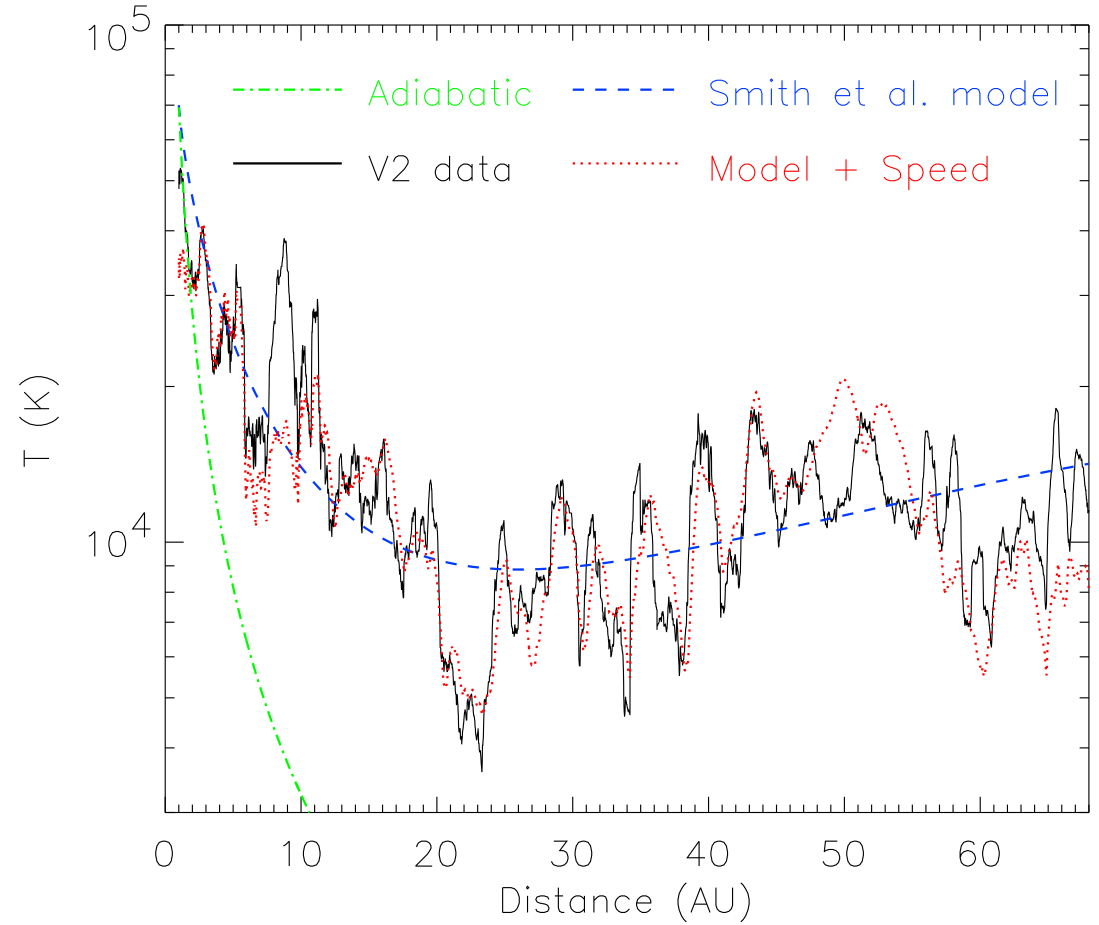
\includegraphics[width=0.8\linewidth,trim=0.5cm 0cm 0cm 0cm, clip=true]{./Part_0/images/heating_profil}
\cprotect\caption{Profil de température ionique en fonction de la distance au Soleil, observé avec les données de Voyager 2 (noir). Profil adiabatique (vert).  Crédits : [\cite{richardson_radial_2003}].}
\label{fig:profil}
\end{figure}
Sur la \figref{fig:profil} est donné l'exemple du profil de température. Du caractère peu collisionnel du vent solaire ont émergé, dans un premier temps, des prédictions d'une décroissance adiabatique du profil de température (courbe verte) [\cite{tu_mhd_1995}]. Comme on peut l'observer, la décroissance n'est pas aussi rapide que le modèle adiabatique. Des exemples de modélisations pour retrouver ce profil sont référencés par [\cite{richardson_radial_2003}]. Sur la \figref{fig:profil}, des résultats d'un modèle prenant en compte des ions dits <<pickups>> sont présentés en bleu et en rouge. Dans le cas rouge, est ajouté au modèle une dépendance linéaire entre la vitesse du vent solaire et la température. Le profil in-situ est ainsi plutôt bien retrouvé mais initialisé à partir de relevés de vitesse et température effectués autour de $\SI{1}{au}$ (unité astronomique dont l'étalon est la distance Soleil-Terre). Les ions pickups font en effet partie des sources du chauffage localisé du vent solaire mais ce chauffage aurait d'autres sources, comme l'explique \cite{david_energy_2022}. 
Avant $\SI{1}{au}$, il serait principalement dû aux fluctuations turbulentes, puis aux chocs interplanétaires venant accélérer ou ralentir le plasma, et enfin, après $\SI{20}{au}$, aux ions pickups provenant du milieu interstellaire. Le chauffage dû aux fluctuations turbulentes est souvent mis en compétition avec un chauffage induit par les processus de reconnexion des lignes de champ magnétique [\cite{matthaeus_who_2011,cranmer_role_2015}]. Ces deux phénomènes sont souvent liés [\cite{sundkvist_dissipation_2007,retino_situ_2007,servidio_magnetic_2011,chasapis_thin_2015,manzini_subion-scale_2023}].  

Dans ces travaux, on s'intéresse au chauffage turbulent [\cite{tu_mhd_1995,kiyani_dissipation_2015}] prédominant à partir de quelques rayons solaires jusqu'à $\SI{2}{au}$. Une définition thermodynamique de ce chauffage sera donnée dans le Chapitre \ref{ch-12}. Ce problème sera abordé à travers la cascade turbulente définie dans le Chapitre \ref{ch-01} et décrite avec une théorie des lois exactes, héritage de la théorie de Kolmogorov. Elle permet un transfert d'énergie des grandes échelles d'injection, à travers les échelles dites fluides et vers les petites échelles (échelles dites cinétiques) où les processus cinétiques dissipatifs peuvent intervenir afin de chauffer les ions et les électrons. 

Ce transfert peut être illustré à partir des spectres d'énergie magnétique comme celui de la \figref{fig:spectre_SW} compilé grâce aux relevés de champ magnétique effectués in-situ par les missions \ac{ACE} et \acs{CLUSTER} en orbite autour de la Terre.  Sur cette figure, on retrouve en fonction de la fréquence temporelle $f$ une pente de type Kolmogorov en $-5/3 \simeq -1.7$. L'hypothèse de Taylor permet de relier le vecteur d'onde $\boldsymbol{k}$ introduit dans le Chapitre \ref{ch-01}, à la fréquence temporelle $f$ accessible dans les relevés in-situ, grâce à la vitesse du vent ($\boldsymbol{v}_{SW}$) : $2 \pi f \sim \boldsymbol{v}_{SW} \cdot \boldsymbol{k}$.
Cette pente indique donc les échelles inertielles et la présence de turbulence dans le plasma d'après la définition spectrale de la zone inertielle donnée dans le Chapitre \ref{ch-01} et transposée à l'énergie magnétique. 
À plus hautes fréquences, cette zone inertielle s'achève par une rupture de pente autour de la fréquence associée à une longueur caractéristique ionique (la longueur d'inertie ($d_i$) ou le rayon de Larmor ($\rho_{Li}$) noté sur la figure $\rho_i$). 
À partir de cette échelle, des effets cinétiques ioniques commencent donc à être visibles. Ensuite, le spectre semble se stabiliser autour d'un nouveau régime a priori dispersif, avec une pente proche de $-2.6$, avant d'atteindre la zone d'influence des électrons autour de la fréquence associée à une longueur caractéristique électronique ($d_e$ ou $\rho_{Le}$, noté sur la figure $\rho_e$). Les phénomènes d'origine cinétique impliqués dans la zone de transition et les zones qui s'ensuivent ne sont pas encore complètement compris, tout comme leurs impacts sur les régimes turbulents (voir par exemple \cite{alexandrova_solar_2013} et \cite{sahraoui_magnetohydrodynamic_2020}). 
\begin{figure}[!ht]
 \centering
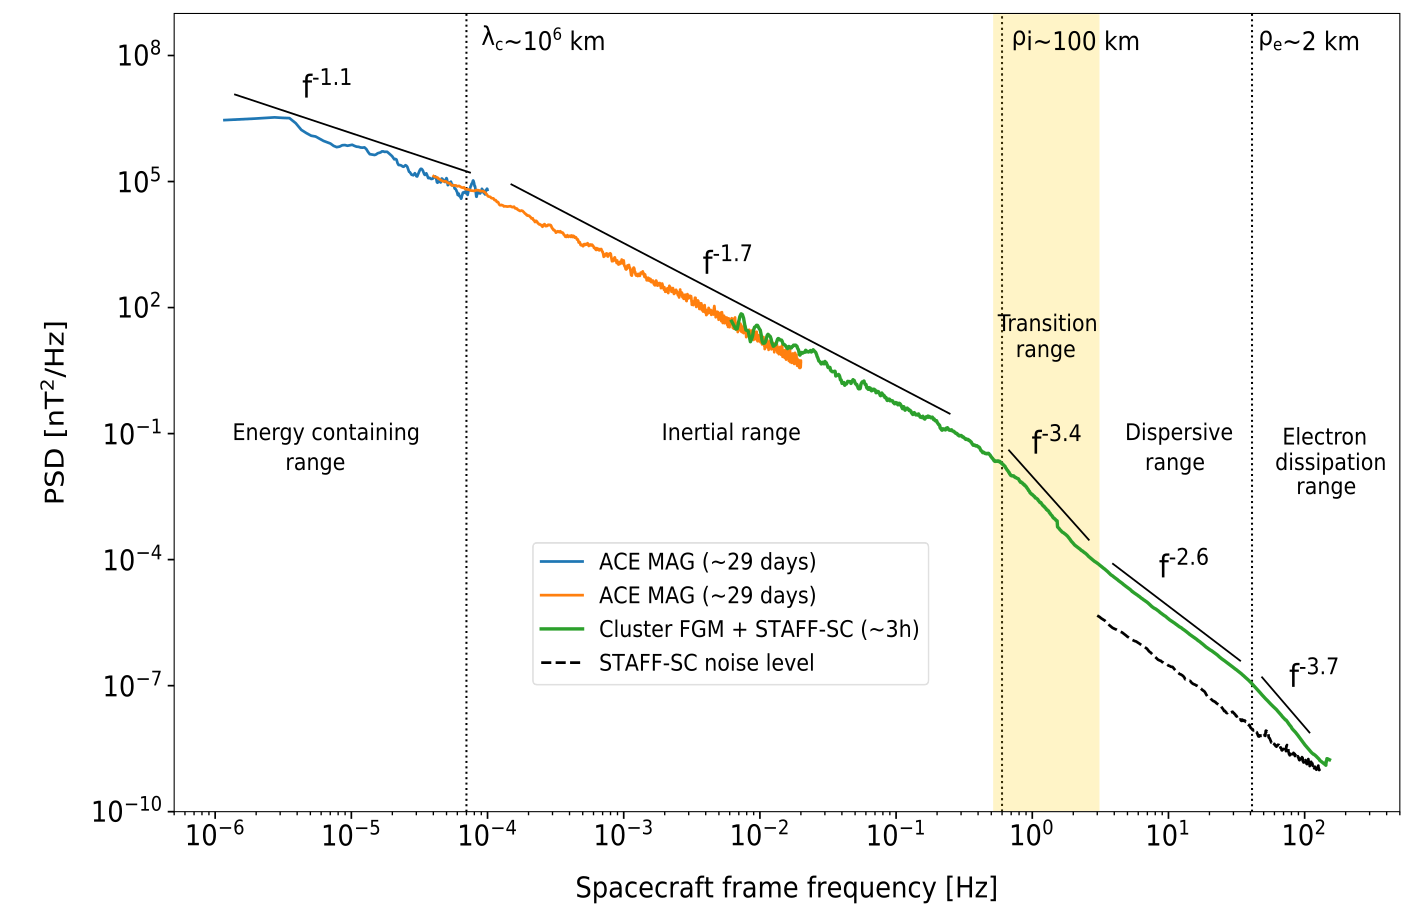
\includegraphics[width=\linewidth,trim=0.5cm 0cm 0cm 0cm, clip=true]{./Part_0/images/spectre_SW}
\cprotect\caption{Spectre d'énergie magnétique du vent solaire obtenu à partir des missions ACE et Cluster. Ce spectre peut être découpé en cinq régions grâce aux ruptures de pentes. Pente en $-1.1$ : Réservoir d'énergie. $\lambda_c$ : longueur de corrélation. Pente en $-1.7$ : Zone inertielle. $\rho_i$ : rayon de Larmor ionique. Pente en $-3.4$ : Zone de transition. Pente en $-2.6$ : Échelles dispersives. $\rho_e$ : rayon de Larmor électronique. Pente en $-3.7$ : Échelles de dissipation électronique. Crédits : [\cite{sahraoui_magnetohydrodynamic_2020}].}
\label{fig:spectre_SW}
\end{figure}

Parmi ces questions ouvertes dans l'étude de la turbulence compressible pour le chauffage du vent solaire, on s'attaquera aux effets conjoints du manque de collision et du champ magnétique sur la cascade. Ces deux propriétés induisent une anisotropie de la fonction de distribution de vitesse des particules, menant à un tenseur de pression anisotrope. Cette anisotropie de pression peut induire des instabilités dans le système [\cite{parker_dynamical_1958,berezin_firehose_1976,hall_firehose_1981,southwood_mirror_1993,gary_proton_1976,hunana_introductory_2019}]. 

La cascade turbulente d'énergie a été largement étudiée dans le cas incompressible depuis le début du siècle et l'extension de la théorie des lois exactes de Kolmogorov au modèle magnétohydrodynamique incompressible par \cite{politano_von_1998} et \cite{politano_dynamical_1998}. Les études sur l'effet de la compression sur la cascade sont quant à elles plus récentes et leur cadre souvent limité par l'hypothèse thermodynamique isotherme [\cite{marino_scaling_2023}]. Dans le Chapitre \ref{ch-11}, nous reprendrons quelques résultats incompressibles avant d'apporter dans la Partie \ref{part_1} une première extension du cadre d'étude de la cascade turbulente à des plasmas compressibles, en centrant la problématique sur l'effet de différentes descriptions thermodynamiques utilisées pour définir la pression. Dans la Partie \ref{part_2}, nous élargirons le cadre de la théorie des lois exactes en prenant en compte l'anisotropie de pression. Dans la Partie \ref{part_3}, nous appliquerons la théorie analytique ainsi élargie à des simulations tridimensionnelles turbulentes. 

Mais, avant cela, dans la section \ref{sec-023}, sera rappelée la description fluide d'un plasma qui sert de base à l'ensemble des modèles utilisés dans ces travaux, et, dans le Chapitre \ref{ch-11}, nous allons introduire la première extension de la théorie de Kolmogorov à un plasma et quelques résultats fondamentaux associés aux plasmas incompressibles. 

\section{Décrire un plasma à l'aide d'un modèle fluide} \label{sec-023}

Soit un plasma, dans lequel chaque particule est caractérisée par le ratio charge/masse, $q_{\alpha}/m_{\alpha}$, associée à son espèce notée $\alpha$, sa position dans l'espace des phases $\{\mathbf{x},\mathbf{v}\}$ et une fonction de distribution $\mathcal{P}_{\alpha}\left(\mathbf{x},\mathbf{v},t\right)$. Dans les cas étudiés ici, les espèces sont les protons ($\alpha = i$) et les électrons ($\alpha=e$). En négligeant les collisions entre les particules, l'équation cinétique, nommée alors équation de Vlasov, décrivant l'évolution de la fonction de distribution des particules est : 
\begin{equation}
\partial_t \mathcal{P}_{\alpha} +  \mathbf{v} \cdot \nabla \cdot \mathcal{P}_{\alpha} + \frac{d \mathbf{v}}{d t} \cdot \nabla_{\mathbf{v}}  \cdot  \mathcal{P}_{\alpha}  = 0.
\label{kinetic vlasov}
\end{equation}
Le système est alors décrit par sept variables, une temporelle $t$, les trois composantes de la position $\mathbf{x}=\left[x,y,z\right]$ associée à l'opérateur dérivatif $\nabla$ et les trois composantes de la vitesse $\mathbf{v}$ associée à l'opérateur dérivatif $\nabla_{\mathbf{v}}$ et dépendante du temps. Si l'on considère que les particules baignent dans un champ électromagnétique $\{\boldsymbol{E}\left(\mathbf{x},t\right),\boldsymbol{B}\left(\mathbf{x},t\right)\}$, on peut remplacer $\frac{d \mathbf{v}}{d t}$  par la force électromagnétique de Lorentz $q_{\alpha}/m_{\alpha} \left(\boldsymbol{E} + \mathbf{v} \times \boldsymbol{B}\right)$ et compléter le système avec les équations de Maxwell :
\begin{eqnarray}
    \label{eq:M1}\nabla \cdot \boldsymbol{E} &=& Q/\epsilon_0 ,\\
     \label{eq:M2}\nabla \cdot \boldsymbol{B} &=& 0 ,\\
     \label{eq:M3}\nabla \times \boldsymbol{E} &=& -\partial_t \boldsymbol{B} ,\\
     \label{eq:M4}\nabla \times \boldsymbol{B} &=& \mu_0 \boldsymbol{j} + \epsilon_0 \mu_0 \partial_t \boldsymbol{E} ,
\end{eqnarray}
avec $Q\left(\mathbf{x},t\right)$ et  $\boldsymbol{j}\left(\mathbf{x},t\right)$ les densités totales de charges et de courant du plasma. 

On peut définir des quantités macroscopiques, des <<moments>> de la fonction de distribution, en moyennant une fonction $g\left(\mathbf{x},\mathbf{v},t\right)$ dans l'espace des vitesses ($d^3v=dv_xdv_ydv_z$) : 
\begin{equation}
 \left<G\left(\mathbf{x},t\right)\right>_{\alpha} = \int^{+\infty}_{-\infty} \mathcal{P}_{\alpha}\left(\mathbf{x},\mathbf{v},t\right) g\left(\mathbf{x},\mathbf{v},t\right) d^3v \, .
\end{equation}
Afin d'appliquer cette moyenne, on supposera la convergence des intégrales. Les étapes de calculs ne seront pas détaillées. Pour plus d'informations, se référer à, par exemple, [\cite{krall_principles_1973,rax_physique_2005,galtier_introduction_2016,belmont_introduction_2018}].
Visuellement, les moments d'ordre 0, sont reliés à l'aire sous la fonction de distribution, ceux d'ordre 1 sont reliés à sa valeur moyenne et ceux d'ordre 2 à sa largeur à mi-hauteur comme représenté sur la \figref{fig:distrib}. 
\begin{figure}[!ht]
 \centering
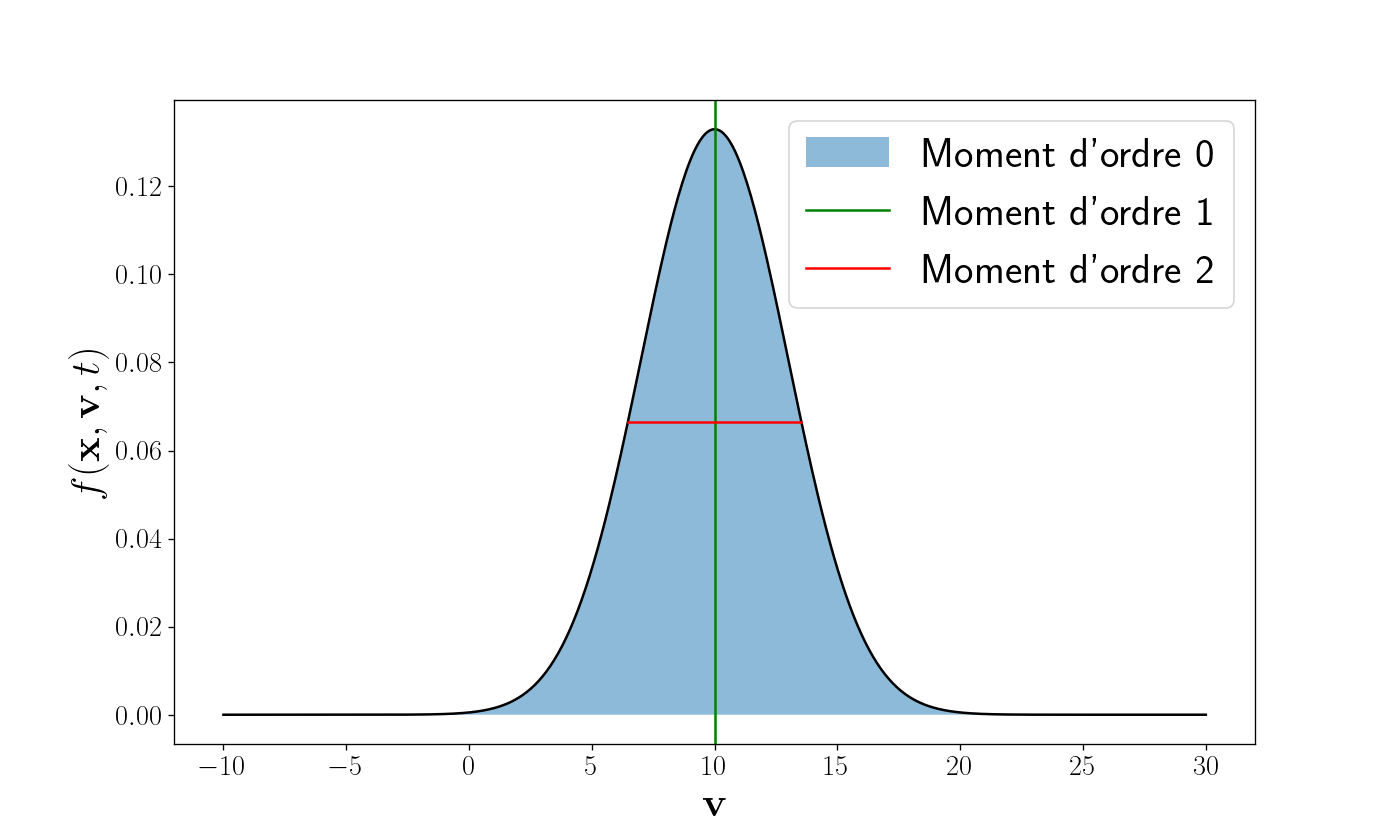
\includegraphics[width=\linewidth,trim=2cm 0cm 3cm 1cm, clip=true]{./Part_0/images/distrib}
\cprotect\caption{Représentation graphique des moments d'ordre 0 (aire sous la courbe colorée en bleu), 1 (valeur moyenne de $\mathbf{v}$ indiquée par la verticale verte) et 2 (largeur indiquée par l'horizontale rouge) de la fonction de distribution en vitesse $f\left(\mathbf{x},\mathbf{v},t\right)$ ici gaussienne.}
\label{fig:distrib}
\end{figure}
 

Suivant la fonction $g$, on peut obtenir pour chaque espèce, les quantités macroscopiques suivantes, aussi appelées <<moments>>,  : 
\begin{table}[!ht]
\begin{center}
\begin{tabular}{ c|c|c|c } 
Quantité & $\left<G\left(\mathbf{x},t\right)\right>_{\alpha}$ & $g\left(\mathbf{x},\mathbf{v},t\right)$  & ordre\\
\hline
Densité de particules & $n_{\alpha}\left(\mathbf{x},t\right)$ & $1$  & 0 \\
Densité de masse & $\rho_{\alpha}\left(\mathbf{x},t\right)$ & $m_{\alpha}\left(\mathbf{x},t\right)$ & 0 \\
Densité de charge & $Q_{\alpha}\left(\mathbf{x},t\right)$ & $q_{\alpha}\left(\mathbf{x},t\right)$ & 0\\
Densité de vitesse du fluide & $n_{\alpha} \boldsymbol{v_{\alpha}}\left(\mathbf{x},t\right)$ & $\mathbf{v}$ & 1\\
Densité de courant & $\boldsymbol{j_{\alpha}}\left(\mathbf{x},t\right)$ & $q_{\alpha} \boldsymbol{v_{\alpha}}$ & 1\\
Pression & $\overline{\boldsymbol{P_{\alpha}}} \left(\mathbf{x},t\right)$ & $m_{\alpha}\left(\mathbf{v}-\boldsymbol{v_{\alpha}}\right)\left(\mathbf{v}-\boldsymbol{v_{\alpha}}\right)$ & 2\\
Flux de chaleur& $\overline{\overline{\boldsymbol{q_{\alpha}}}}\left(\mathbf{x},t\right)$ & $m_{\alpha}\left(\mathbf{v}-\boldsymbol{v_{\alpha}}\right)\left(\mathbf{v}-\boldsymbol{v_{\alpha}}\right)\left(\mathbf{v}-\boldsymbol{v_{\alpha}}\right)$ & 3\\
\end{tabular}
\end{center}
\end{table}

À partir de l'équation de Vlasov, on obtient des équations dites <<multi-fluides>> (dépendantes de $\alpha$) décrivant l'évolution des différents moments :
\begin{itemize}
    \item L'équation de continuité pour la densité massique :
\begin{eqnarray}
  \label{eq:model_0_multi} \partial_t \rho_{\alpha} + \nabla \cdot \left(\rho_{\alpha} \boldsymbol{v_{\alpha}}\right) &=& 0.
 \end{eqnarray}
    \item L'équation sur la quantité de mouvement :
\begin{eqnarray}
  \label{eq:model_1_multi} \partial_t \left(\rho_{\alpha} \boldsymbol{v_{\alpha}}\right) + \nabla \cdot \left(\rho_{\alpha} \boldsymbol{v_{\alpha}}\boldsymbol{v_{\alpha}} + \overline{\boldsymbol{P_{\alpha}}}\right) - Q_{\alpha} \boldsymbol{E} - \boldsymbol{j_{\alpha}} \times \boldsymbol{B} &=& 0.
 \end{eqnarray}
 \item L'équation d'évolution du tenseur de pression :
\begin{eqnarray}
  \label{eq:model_2_multi} \partial_t \overline{\boldsymbol{P_{\alpha}}} + \nabla \cdot \left(\boldsymbol{v_{\alpha}}\overline{\boldsymbol{P_{\alpha}}} + \overline{\overline{\boldsymbol{q_{\alpha}}}}\right) + \left(\overline{\boldsymbol{P_{\alpha}}} \cdot \nabla \boldsymbol{v_{\alpha}}\right)^S +  \frac{Q_{\alpha}}{\rho_{\alpha}} \left(\boldsymbol{B}\times \overline{\boldsymbol{P_{\alpha}}}\right)^S  &=& 0 ,
\end{eqnarray}
\end{itemize}
avec $\left( \right)^S = \left( \right) + \left( \right)^T$ avec $\left( \right)^T$ la transposée de $\left( \right)$. Ces équations sont associées respectivement aux moments d'ordre 0, 1 et 2. On remarque que l'équation du moment d'ordre $n$ dépend d'un moment d'ordre $n+1$. Afin de fermer le système d'équations, des équations dites <<de fermeture>>, devront être introduites. 

Dans les plasmas que l'on considère, on a deux populations ($\alpha = i,e$): les ions/protons ($m_i$, $e$) et les électrons ($m_e$, $-e$) avec les masses $m_i \gg m_e$ et $e$ la charge élémentaire. Le système d'équation multi-fluide sera donc appelé <<bi-fluide>>. On l'abordera dans le Chapitre \ref{ch-23}. 

Les quantités totales (notées sans indices : $n$, $\rho$, $\boldsymbol{v}$, $\boldsymbol{j}$, etc.) sont ensuite obtenues en sommant sur toutes les espèces, $n_{\alpha}$, $\rho_{\alpha}$, $Q_{\alpha}$, $\rho_{\alpha} \boldsymbol{v_{\alpha}}$, $\boldsymbol{j_{\alpha}}$, $\overline{\boldsymbol{P_{\alpha}}} +  \rho_{\alpha} \boldsymbol{v_{\alpha}}\boldsymbol{v_{\alpha}}$ et $\rho_{\alpha} u_{\alpha} + \frac{1}{2} \rho_{\alpha} |\boldsymbol{v_{\alpha}}|^2$.  En appliquant ces sommations aux équations \eqref{eq:model_0_multi}, \eqref{eq:model_1_multi} et \eqref{eq:model_2_multi} et en considérant l'hypothèse de quasi-neutralité ($Q \simeq 0$), on obtient les équations mono-fluides quasi-neutres suivantes :
\begin{itemize}
    \item L'équation de continuité pour la densité massique :
\begin{eqnarray}
  \label{eq:model_0_mono} \Rightarrow \partial_t \rho + \nabla \cdot \left(\rho \boldsymbol{v}\right) &=& 0 .
 \end{eqnarray}
    \item L'équation sur la quantité de mouvement :
\begin{eqnarray}
\label{eq:model_1_mono} \Rightarrow \partial_t \left(\rho \boldsymbol{v}\right) + \nabla \cdot \left(\rho \boldsymbol{v}\boldsymbol{v} + \overline{\boldsymbol{P}}\right) - \boldsymbol{j} \times \boldsymbol{B} &=& 0 .
 \end{eqnarray}
 \item L'équation d'évolution du tenseur de pression, avec $\overline{\boldsymbol{P_E}} = \sum_{\alpha} \frac{Q_{\alpha}}{\rho_{\alpha}} \overline{\boldsymbol{P_{\alpha}}}$ :
\begin{eqnarray}
 \label{eq:model_2_mono} \Rightarrow \partial_t \overline{\boldsymbol{P}} + \nabla \cdot \left(\boldsymbol{v}\overline{\boldsymbol{P}} + \overline{\overline{\boldsymbol{q}}}\right) + \left(\overline{\boldsymbol{P}} \cdot \nabla \boldsymbol{v}\right)^S +  \frac{Q}{\rho} \left(\boldsymbol{B}\times \overline{\boldsymbol{P_E}}\right)^S  &=& 0 .
\end{eqnarray}
\end{itemize}
L'hypothèse non-relativiste et la quasi-neutralité permettent d'y remplacer $\boldsymbol{j}$ par $\nabla \times \boldsymbol{B}$ (Equation de Maxwell \eqref{eq:M4}).

On peut construire, à partir de l'équation \eqref{eq:model_1_multi}, l'équation d'évolution de la densité de courant totale $\boldsymbol{j} = e n_i \boldsymbol{v_i} - e n_e \boldsymbol{v_e}$. Sachant que $m_i \gg m_e$, cette équation peut s'écrire sous la forme de la loi d'Ohm généralisée : \begin{equation} 
\boldsymbol{E} =  \boldsymbol{E_{ind}} +  \boldsymbol{E_{hall}} +  \boldsymbol{E_{therm}} \label{eq:ohm} 
\end{equation}
avec :
\begin{itemize}
 \item $\boldsymbol{E_{MHD}} =  - \boldsymbol{v} \times \boldsymbol{B}$, le terme d'induction,
 \item $\boldsymbol{E_{hall}} = \lambda_i \frac{\boldsymbol{j}}{\rho} \times \boldsymbol{B}$, le terme de \acl{Hall},
 \item $\boldsymbol{E_{\nabla P_e}} = - \frac{\lambda_i}{\rho} \nabla \cdot \overline{\boldsymbol{P_{e}}}$,  \acl{Pe},
\end{itemize}
avec $\lambda_i = \frac{m_i}{e}$. La loi d'Ohm permet d'expliciter $\boldsymbol{E}$ dans l'équation \eqref{eq:M3}. En ne prenant en compte que le terme d'induction dans la loi d'Ohm, on obtient l'équation : 
\begin{equation}
    \label{eq:model_M3_ideal} \partial_t \boldsymbol{B} = \nabla \times \left(\boldsymbol{v} \times \boldsymbol{B} \right)
\end{equation}
qui s'écrit en fonction de la vitesse d'Alfvén $\boldsymbol{v_A} = \frac{\boldsymbol{B}}{\sqrt{\mu_0 \rho}}$ avec $\mu_0$, la perméabilité du vide, : 
\begin{equation}
\label{eq:model_M3_idealvA} \partial_t \boldsymbol{v_A}  =   \nabla \cdot \left(\boldsymbol{v_A}\boldsymbol{v} - \boldsymbol{v}\boldsymbol{v_A}\right) -  \boldsymbol{v}  \nabla \cdot \boldsymbol{v_A} +  \frac{\boldsymbol{v_A}}{2}  \nabla \cdot \boldsymbol{v}. \end{equation}

Les équations \eqref{eq:model_0_mono}, \eqref{eq:model_1_mono} avec l'hypothèse non-relativiste, \eqref{eq:model_2_mono} et  \eqref{eq:model_M3_ideal} forment le modèle \ac{MHD} non fermé, valable pour des échelles temporelles associées à des fréquences plus petites que la fréquence cyclotron ionique $\omega_{ci} = B_0/\lambda_i$ avec $B_0 = \left<|\boldsymbol{B}|\right>$ et des échelles spatiales, dites \ac{MHD}, plus grandes que $d_i$ et $\rho_{Li}$. En fonction de l'équation de fermeture choisie, l'équation \eqref{eq:model_2_mono} peut être omise, par exemple dans le cas d'une fermeture isotherme où $\overline{\boldsymbol{P}} \propto \rho$.
Usuellement, la pression est supposée isotrope dans le modèle \acs{MHD} mais dans ce mémoire, on ne fera cette hypothèse que dans la Partie \ref{part_1}. Dans la Partie \ref{part_2}, on abordera l'extension de la théorie des lois exactes au modèle \acs{MHDH} pour laquelle l'équation d'induction peut s'écrire : 
\begin{equation}
\partial_t \boldsymbol{v_A}  =   \nabla \cdot \left(\boldsymbol{v_A}\boldsymbol{v} - \boldsymbol{v}\boldsymbol{v_A}\right) -  \boldsymbol{v}  \nabla \cdot \boldsymbol{v_A} +  \frac{\boldsymbol{v_A}}{2}  \nabla \cdot \boldsymbol{v} - \frac{\lambda}{ \sqrt{\rho} } \nabla \times\left(\frac{1}{\sqrt{\rho}} \boldsymbol{j}\times \boldsymbol{v_A}\right)  .\label{eq:model_M3_hall}
\end{equation}
Ce modèle est souvent normalisé par la vitesse d'Alfvén moyenne $v_{A0}$. Dans l'équation \eqref{eq:model_M3_hall}, $\lambda_i$ est alors remplacée par la longueur inertielle des ions $d_i = v_{A0}\omega_{ci}$. Ce modèle sera donc valable aux échelles MHD et aux échelles dites Hall, proches de $d_i$. Certaines simulations que l'on analysera dans la Partie \ref{part_3} prennent aussi en compte le \acl{Pe}. Nous proposerons donc une extension au modèle \acs{MHDHPe}. Ce terme permet de prendre en compte la contribution thermique des électrons au champ électrique. 
%Le terme inertiel électronique, dépendant de $\lambda_e$, permet quant à lui d'accéder aux échelles électroniques proches de $d_e$ ou $\rho_{Le}$.

\section{Synthèse : problématique et modèles utilisés}
\label{synt-02}
\fcolorbox{red}{white}{\begin{minipage}[c]{\linewidth}
\paragraph{Problématique générale : } Quel est l'impact des fermetures dépendant de la pression sur la cascade turbulente ? \\

\paragraph{Plan : }
\begin{itemize}
    \item Partie \ref{part_1} : Impact d'une pression isotrope sur la cascade turbulente compressible,
    \item Partie \ref{part_2} : Description d'un écoulement turbulent dépendant d'une pression anisotrope,
    \item Partie \ref{part_3} : Effet de l'anisotropie de pression sur la cascade turbulente. \\
\end{itemize}
\end{minipage}}

\fcolorbox{blue}{white}{\begin{minipage}[c]{\linewidth}

\paragraph{Modèles utilisés}
\begin{eqnarray}
  \label{eq:synth_model_0_mono} \Rightarrow \partial_t \rho + \nabla \cdot \left(\rho \boldsymbol{v}\right) &=& 0 \\
\label{eq:synth_model_1_mono} \Rightarrow \partial_t \left(\rho \boldsymbol{v}\right) + \nabla \cdot \left(\rho \boldsymbol{v}\boldsymbol{v} + \overline{\boldsymbol{P}}\right) - \boldsymbol{j} \times \boldsymbol{B} &=& 0 \\
 \label{eq:synth_model_2_mono} \Rightarrow \partial_t \overline{\boldsymbol{P}} + \nabla \cdot \left(\boldsymbol{v}\overline{\boldsymbol{P}} + \overline{\overline{\boldsymbol{q}}}\right) + \left(\overline{\boldsymbol{P}} \cdot \nabla \boldsymbol{v}\right)^S +  \left(\boldsymbol{B}\times \overline{\boldsymbol{P_E}}\right)^S  &=& 0 
\end{eqnarray}
\begin{itemize}
\item \ac{MHD} (Parties \ref{part_1} et \ref{part_2}) : 
\begin{equation}
    \label{eq:synth_M3_ideal} \partial_t \boldsymbol{B} = \nabla \times \left(\boldsymbol{v} \times \boldsymbol{B} \right)
\end{equation}
\item \acs{MHDH} (Parties \ref{part_2} et \ref{part_3}) : 
\begin{equation}
    \label{eq:synth_M3_hall} \partial_t \boldsymbol{B} = \nabla \times \left(\boldsymbol{v} \times \boldsymbol{B} \right) - \lambda \nabla \times \left( \frac{\boldsymbol{j}}{\rho} \times \boldsymbol{B} \right)
\end{equation}
\item \acs{MHDHPe} (Parties \ref{part_2} et \ref{part_3}) : 
\begin{equation}
    \label{eq:synth_M3_gpe} \partial_t \boldsymbol{B} = \nabla \times \left(\boldsymbol{v} \times \boldsymbol{B} \right) - \lambda \nabla \times \left( \frac{\boldsymbol{j}}{\rho} \times \boldsymbol{B} \right) + \lambda \nabla \times \left( \frac{1}{\rho} \nabla \cdot \overline{\boldsymbol{P_{e}}}\right)
\end{equation}
\item Autre : Bi-fluide (Parties \ref{part_2})\\
\end{itemize}

\end{minipage}}
